\section{Evaluation}

We evaluate our split and merge error detection and correction recommendation in two ways: as an automatic pipeline, and as a proofreading tool to direct users to regions with a high probability of error and to suggest corrections (Fig.~\ref{fig:results}). For comparison, we take publicly available mouse cortex data of the same kind as our training data. This data is part of the ISBI 2013 challenge training dataset ($1024\times1024\times100$ voxels) which was acquired using a serial section scanning electron microscope (ssSEM) with a resolution of $6\times6\times30\, nm$ per voxel. We use the available manually-labeled ground truth to score our approach using the variation of information (VI) metric, which is closely related to mutual information. VI is a measure of the distance between two clusterings, where lower VI numbers are better. Since our classifiers are trained on 2D image slices, we perform all evaluations on slices rather than 3D volumes. \JT{WHICH NETWORK}

\paragraph{Automatic correction.} During training, we define a probability threshold $p_t=.95$ \VKF{This is actually different than the 0.7 claimed before} for automatic split correction based on CNN probability from the test set. Then, for automatic correction, we apply both classifiers to produce lists of split and merge errors sorted by confidence. First, we correct merge errors with $\max(1-p)$, followed by split error correction using $p_t$. The total time for the correcting all \JT{\#} errors was 17 minutes (\JT{\#} merge error correction 15min, \JT{\#} split error correction 2min). The average VI improvement in comparison to the ground truth was \VKF{update} (Fig.~\ref{fig:results}).
% errors was 17 minutes, 

\paragraph{Interactive proofreading.}
Recently, Haehn et al.~discussed requirements for interactive proofreading and evaluated three different tools on connectomics data in a study with naive users~\cite{haehn_dojo_2014}. %The authors performed a non-expert user study and stated that their software Dojo provides better results than other tools due to a minimalistic user interface and sophisticated 3D volume rendering. 
This study asked users to spend 30 minutes proofreading with the different tools, to correct split and merge errors to improve the automatic segmentation. We use their findings as baseline for the evaluation of our method.

\VKF{This should go together with the other data description. Not going back myself because of git.}


which is the same kind of data as our training data and user-generated proofreading result data LINK MISSING.
Haehn et al. perform their user study on the most representative sub-volume ($400\times400\times10$ voxels) in terms of distribution of object size. For optimal comparison, we use exactly the same data.

\JT{Up to here.}
\textbf{User-guided proofreading.} For the evaluation of user-guided proofreading, we simulate user feedback during our automatic correction by comparing the resulting segmentation before and after each performed correction to the ground truth segmentation. Since users are not perfect, we also introduce an error rate which simulates falsely specified user feedback. This error rate defines if we accept a good split or reject it as well as accept a bad split or reject such, based on direct comparison with the ground truth using a scoring metric. Assuming a perfect user with an error rate of 0, the average VI improvement in comparison to the ground truth was \VKF{update $0.11$}.

\textbf{Interactive proofreading.} We use the published results from Haehn et al. to compare our results against fully interactive proofreading using their software Dojo. In this study, the proofreading time was limited to 30 minutes and participants performed 59 corrections on average (~30 seconds per correction). For our interactive proofreading we assume that  non-experts can perform a correction using our system in 15 seconds, as they only have to accept or reject the suggested solution, instead of drawing correction boundaries for merge errors or clicking on relevant regions for split errors in Dojo. 

Since the performance between participants of Haehn's user study shows large differences, we decided to choose the best performing user (VI improvement $.0598$) as well as the average performance among all users (VI improvement $-0.012$) as our baseline.

\begin{figure}[t]
\centering
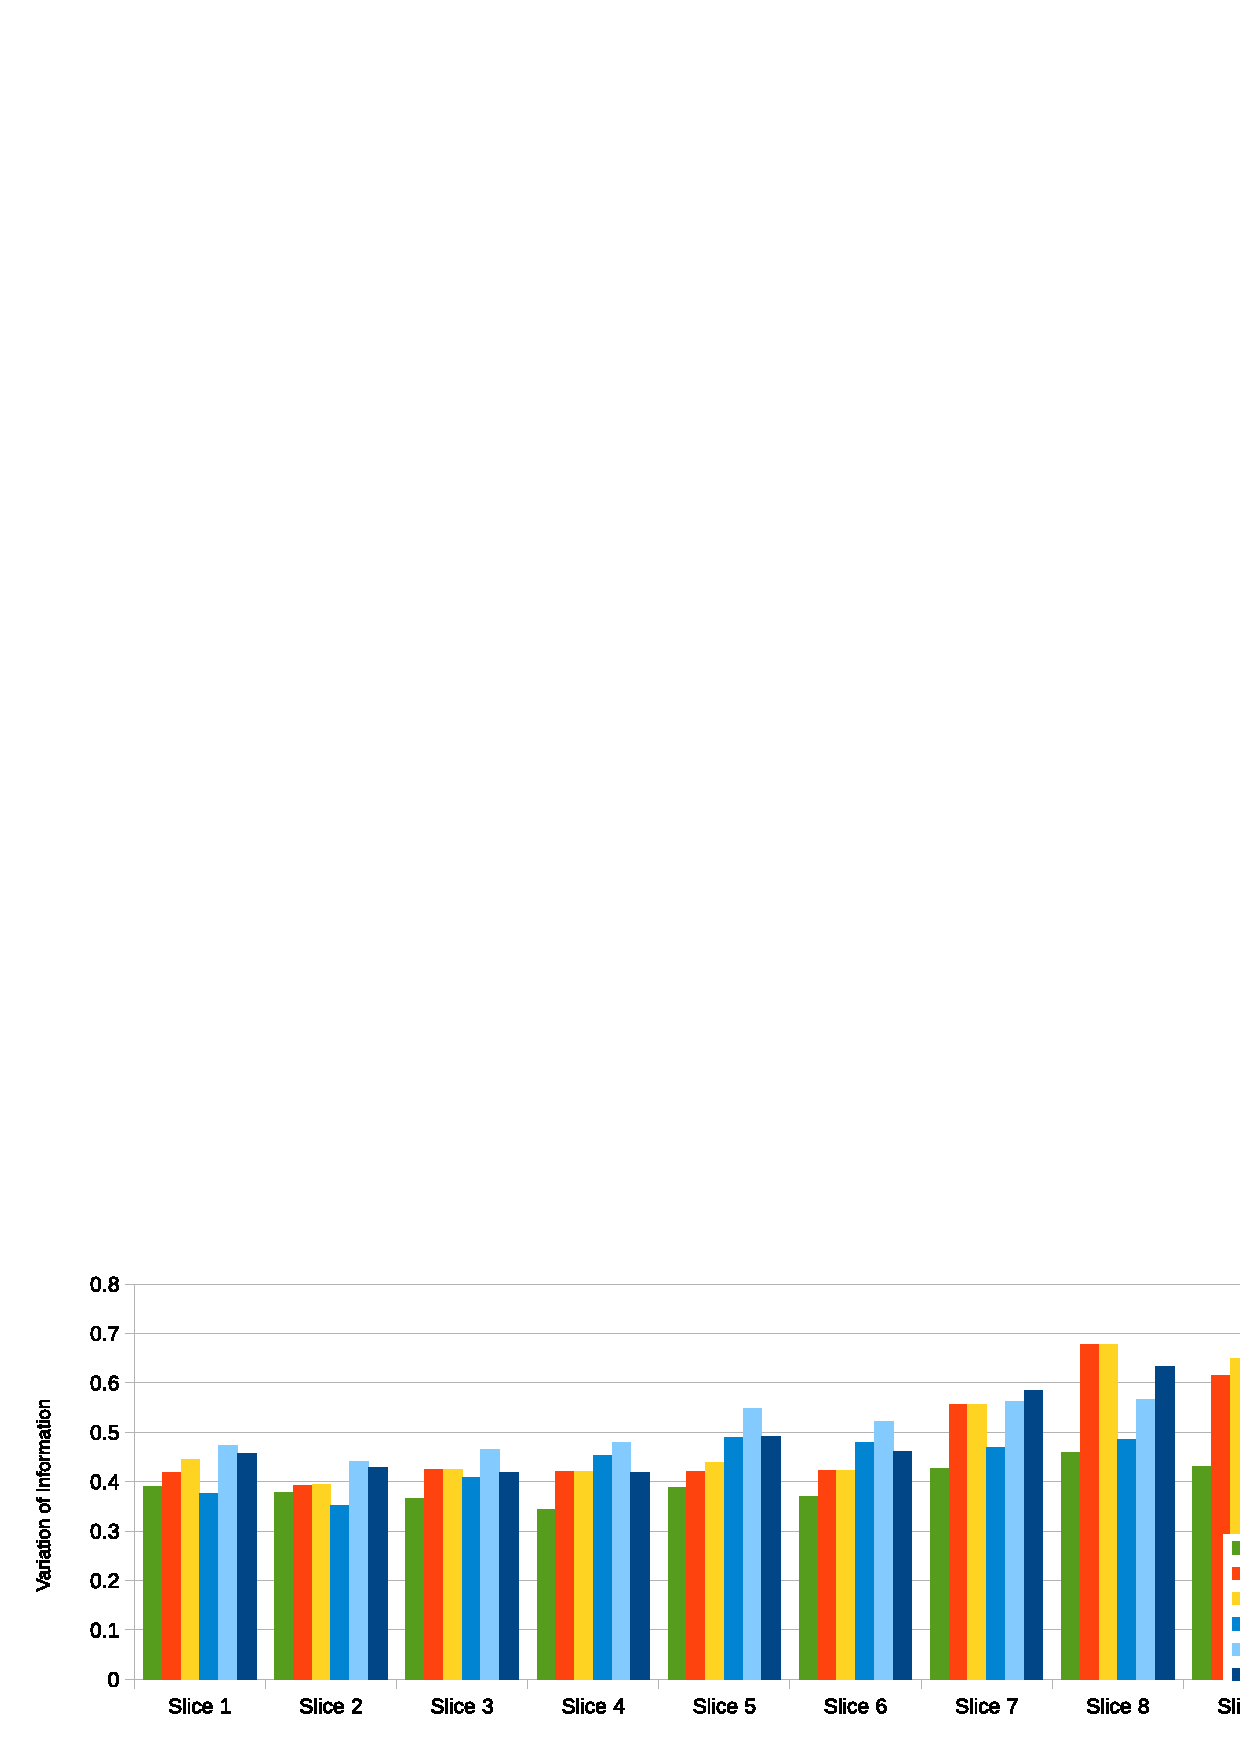
\includegraphics[scale=.45]{gfx/results.pdf}
\caption{We compare user-guided (error rate 0.0) and automatic (full+just splits) proofreading results using our trained network,  as well as results from Haehn et al.'s comparison study \cite{haehn_dojo_2014} across 2D slices of connectomics data. The score is measured in variation of information (VI) between an input and the corresponding performance. Lower scores are better.}
\label{fig:results}
\end{figure}
%
%
%\subsection{Split error evaluation}
%
%Paragraph: What is the process of evaluating split errors?
%
%Paragraph: What do we compare against? What is the result? Why is the performance better?
%
%\begin{table}[t]
%\begin{tabular}{ll}
%\toprule
%Method & VI improvement after fixing split errors \\
%\midrule
%Jain design & \\
%Jain design variation & \\
%Our design &  \\
%Our design variation & \\
%\bottomrule
%\end{tabular}
%\caption{This is a table of results. It shows the comparison to Jain et al., and the comparison to different variations of these algorithms with the varying overlap regions.}
%\label{tab:spliterrorcorrectionperformance}
%\end{table}
%
%\subsubsection{Analysis}
%
%Paragraph: Demonstration of ROC curves for VI performance in split error adjustment as the threshold varies.
%
%\begin{figure}[t]
%\missingfigure{}
%\caption{What does the performance of split error correction look like (ROC curve) as the threshold on edge probability changes?}
%\end{figure}
%
%\subsection{Merge error evaluation}
%
%Merge errors are not that common. False positive rate is very important. Choosing threshold is important.
%
%Paragraph: What is the process of evaluating merge errors?
%
%Paragraph: What do we compare against? What is the result? Why is the performance better?
%
%\begin{table}[t]
%\begin{tabular}{ll}
%\toprule
%Method & VI improvement after fixing merge errors \\
%\midrule
%Our design &  \\
%Our design variation & \\
%\bottomrule
%\end{tabular}
%\caption{This is a table of results. It shows our ability to improve VI.}
%\end{table}
%
%
%
%Philosophical point of trading split errors for merge errors...
%
%
%Speed of classification